\documentclass{article}
\begin{document}

\section{Experimental setup}

\begin{figure}[H]
	\centering
	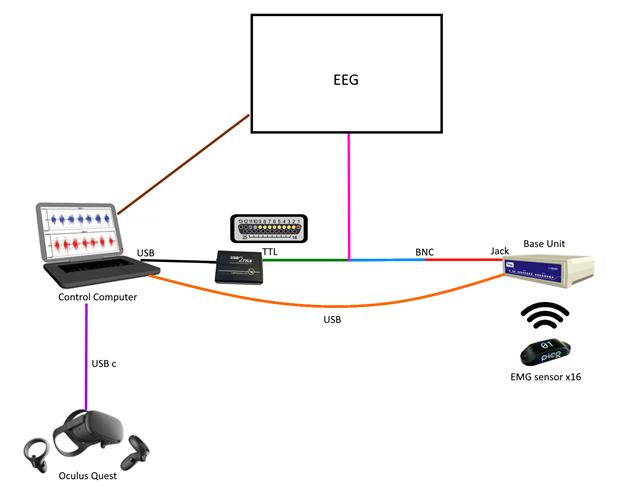
\includegraphics[width=10cm]{images/experimentalSetup.png}
	\caption{Diagram of the experimental setup for data collection}
	\label{fig:experimentalSetup}
\end{figure}


\section{Hand gesture data collection from the Oculus Quest}

In this section, we describe the development of a Unity project that can be executed on the Oculus Quest headset to collect hand motion data. The first part of this software is the setup of the OVR library in a new Unity 3D project. When this project is built in an APK file and loaded on the Oculus Quest, it can already display the user hands using motion tracking.

\subsection{Data collection}

A $C\#$ script called $dataSaving.cs$ is placed in the Unity scene to record all the information of the motion tracking. This script has a function $FixedUpdate()$ which is called by the engine with a regular period (set to a frequency of 50Hz to match the motion tracking frequency). This function has access to the scripts $OVRSkeleton$ and $OVRHand$ of both hands which contain the information on a current hand gesture. It can also get the variable $System.DateTime.UtcNow.Ticks$ to get the UTC of the frame, which will be later used for synchronization.

All the collected data is appended in a csv file (with $";"$ separator) where each line represent a single frame. A description of this file is given below.

\begin{table}[H]
	\centering
	\begin{tabular}{|c|p{12cm}|}
		\hline
		Column index & data \\
		\hline
		1 & UTC \\ \hline
		2 & Boolean telling if the whole data of the left hand is valid \\ \hline
		3 & Position (x, y, z) and rotation (x, y, z) of the left hand in the 3D space \\ \hline
		4 - 22 & Rotation (x, y, z) of 19 bones of the left hand \\ \hline
		23 - 26 & Boolean telling if the fingers 2 to 5 of the left hand are touching the thumb of the left hand (pinching action) \\ \hline
		27 - 31 & Boolean telling if the confidence in the quality of the pose estimation of the finger 1 to 5 is high or low \\ \hline
		32 - 61 & Same as 2 - 31 but for the right hand \\ \hline
		62 & Name of the gesture recognized by the library \textit{Hand Tracking Gesture  Recorder} (\url{https://github.com/jorgejgnz/HandTrackingGestureRecorder}) among those recorded for the right hand\\
		\hline
	\end{tabular}
	\caption{Caption}
	\label{tab:my_label}
\end{table}

The indexes of the fingers are:
\begin{enumerate}
	\item Thumb
	\item Index
	\item Middle
	\item Ring
	\item Pinky
\end{enumerate}

The indexed of each finger bone can be found in the documentation of the OVR library (\url{https://developer.oculus.com/documentation/unity/unity-handtracking/}) and is described in figure \ref{fig:ovrHandIndexesTab} and shown in figure \ref{fig:ovrHandIndexes}.

\begin{figure}[h]
	\centering
	\begin{verbatim}
	Hand_WristRoot   = Hand_Start + 0 // root frame of the hand, where the wrist is located
	Hand_ForearmStub = Hand_Start + 1 // frame for user's forearm
	Hand_Thumb0      = Hand_Start + 2 // thumb trapezium bone
	Hand_Thumb1      = Hand_Start + 3 // thumb metacarpal bone
	Hand_Thumb2      = Hand_Start + 4 // thumb proximal phalange bone
	Hand_Thumb3      = Hand_Start + 5 // thumb distal phalange bone
	Hand_Index1      = Hand_Start + 6 // index proximal phalange bone
	Hand_Index2      = Hand_Start + 7 // index intermediate phalange bone
	Hand_Index3      = Hand_Start + 8 // index distal phalange bone
	Hand_Middle1     = Hand_Start + 9 // middle proximal phalange bone
	Hand_Middle2     = Hand_Start + 10 // middle intermediate phalange bone
	Hand_Middle3     = Hand_Start + 11 // middle distal phalange bone
	Hand_Ring1       = Hand_Start + 12 // ring proximal phalange bone
	Hand_Ring2       = Hand_Start + 13 // ring intermediate phalange bone
	Hand_Ring3       = Hand_Start + 14 // ring distal phalange bone
	Hand_Pinky0      = Hand_Start + 15 // pinky metacarpal bone
	Hand_Pinky1      = Hand_Start + 16 // pinky proximal phalange bone
	Hand_Pinky2      = Hand_Start + 17 // pinky intermediate phalange bone
	Hand_Pinky3      = Hand_Start + 18 // pinky distal phalange bone
	\end{verbatim}
	\caption{Indexes of the ones of the OVR hand as given by the OVR library}
	\label{fig:ovrHandIndexesTab}
\end{figure}

\begin{figure}[H]
	\centering
	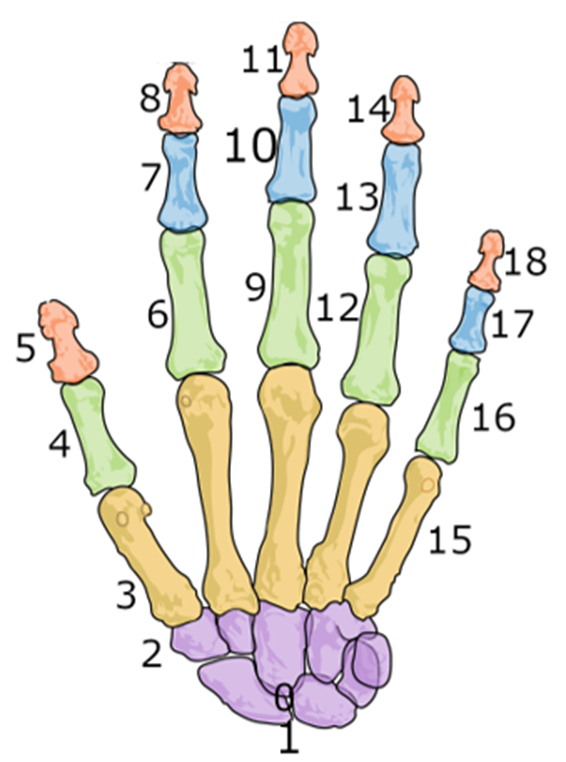
\includegraphics[width=7cm]{images/ovrHandBonesIndexes.png}
	\caption{Graphical representation of the indexes of the ones of the OVR hand as given by the OVR library (\url{https://www.reddit.com/r/OculusQuest/comments/edkp9i/visual_reference_for_hand_tracking_bone_ids/})}
	\label{fig:ovrHandIndexes}
\end{figure}

This is saved in a local file on the Oculus Quest and can be exported to an external computer after the recording using an USB-c link.


\subsection{Remote control}

The experimental setup is made so that the subject does not have to do anything else than the recorded hand gestures. In order to do that, a remote control interface was implemented. It enables to send messages to the Unity program running on the Oculus Quest from an external computer using a USB-c link. Theses messages take the form of files that are pushed in a particular directory, and with a name giving to the action to perform, using \textit{Android Debug Bridge} (ADB: \url{https://developer.android.com/studio/command-line/adb}).

A python script called $remoteControl.py$ was implemented to give an interface to remotely control the Oculus Quest behaviour. The actions that can be done are
\begin{itemize}
	\item Start and stop the recording of the hand motion. A sphere in the 3D Unity scene, seen from the Oculus Quest, changes color to indicate if the recording is activated (red=off, green=on). Stopping the recording also pulls the record file on the computer running this script.
	\item Reset the recording
	\item Save the current gesture of the right hand for the Hand Tracking Gesture  Recorder library
	\item Export the saved right hand gesture in a file (local on the Oculus Quest)
	\item Import the right hand gesture from a file (local on the external computer)
	\item Show the next instruction to the user (described later in the document)
\end{itemize}

\subsection{Interface}




\section{Data synchronization}

An important point of the data set creation is the synchronization of the hand kinematics with the EMG and EEG signals. To perform this synchronization, we make three assumptions on the setup.
\begin{enumerate}
	\item The recording of the EMG and EEG can be started using a trigger signal with a known delay
	\item The timestamps given by the EMG, EEG
	\item The UTC of the external computer and those of the Oculus Quest are synchronized
\end{enumerate}
The 2 first assumptions are relying on the official user manuals of the hardware. We know that the Cometa EMG has a starting delay of 14ms when using a triggered start. The delay for the EEG is \color{red} [TO FIND] \color{black}. The EEG cannot be started with a trigger but it can include the trigger timestamp in its recorded data. So, we just have to cut the data before the first trigger.

To verify the third assumption, we can use the software \textit{SideQuest} (\url{https://sidequestvr.com/}) that enables to stream the screen of the Oculus Quest on a computer using a USB-c cable (called Oculus Link). By doing so, we find a shift of approximately 22ms in average with a standart deviation around 100ms between the computers UTC and the Oculus Quests UTC. This time lag corresponds to the known delay of the SideQuest streaming (\url{https://www.mdpi.com/2073-431X/9/4/92}) which allows us to conclude that they are synchronized.

The algorithm to synchronize the data from the external computer is the following:
\begin{enumerate}
	\item Start the hand motion recording (which takes unknown time) and EEG recording
	\item Wait for the Oculus Quest to send a feedback that its recording has started
	\item Save the current UTC
	\item Send a trigger start signal on the EMG recorder and the EEG recorder
	\item Collect the data until the end of the recording
	\item stop all recording (they might not end exactly at the same time but the timestamps in each part of the records removes the need for synchronized end of record)
	\item Cut the start of the hand kinematics recording at the UTC of the starting of the EMG/EEG recording
	\item Convert the UTC in the hand kinematic file to timestamps in ms starting from 0 (0 corresponds to the UTC saved at the beginning of the recording but there might not be a recorded frame at this exact moment)
	\item Shift the EMG recording by 14ms
	\item Shift the EEG recording by \color{red} [TO FIND] \color{black}
	\item Cut the beginning of the EEG recording (before the first trigger)
	\item place everything in a common folder
\end{enumerate}

\end{document}